\newpage
\section{Approximating NURBS parametrizations with B-spline parametrizations}
\label{Sec2:NURBStransformation}
Starting with any NURBS parametrizations of a geometry where every internal knot has multiplicity $m=\check{p}_\upxi$ in the $\xi$-direction and correspondingly in the other two parameter directions, we want to transform the NURBS parametrization of the exact geometry, to a B-spline representation. This representation approximates the geometry by interpolating the geometry at $n_\upxi\cdot n_\upeta\cdot n_\upzeta$ (not necessarily unique) physical points resulting from a grid in the parametric space.

Let $\vec{X}$ be the NURBS parametrization of the geometry
\begin{equation}
	\vec{X}(\xi,\eta,\zeta) = \sum_{i=1}^{n_\upxi}\sum_{j=1}^{n_\upeta}\sum_{l=1}^{n_\upzeta} R_{i,j,l}(\xi,\eta,\zeta)\vec{P}_{i,j,l},
\end{equation}
with knot vectors $\Xi$, $\Eta$ and $\Zeta$, polynomial order $\check{p}_\upxi$, $\check{p}_\upeta$ and $\check{p}_\upzeta$. For each control point $\vec{P}_{i,j,l}$ we will need a corresponding interpolating point $\vec{Q}_{i,j,l}$ which will be located at the grid point $\left(\tilde{\xi}_i,\tilde{\eta}_j,\tilde{\zeta}_l\right)$. These points in the parameter domain are chosen to be the Greville abscissae
\begin{align}
	\tilde{\xi}_i &= \frac{1}{\check{p}_\upxi}\sum_{\tilde{i} = i+1}^{i+\check{p}_\upxi} \xi_{\tilde{i}},\quad i = 1,\dots, n_\upxi\\
	\tilde{\eta}_j &= \frac{1}{\check{p}_\upeta}\sum_{\tilde{j} = j+1}^{j+\check{p}_\upeta} \eta_{\tilde{j}},\quad j = 1,\dots, n_\upeta\\
	\tilde{\zeta}_l &= \frac{1}{\check{p}_\upzeta}\sum_{\tilde{l} = l+1}^{l+\check{p}_\upzeta} \zeta_{\tilde{l}},\quad l = 1,\dots, n_\upzeta,
\end{align}
where $\xi_i$, $\eta_j$ and $\zeta_l$ are the knots of the knot vectors $\Xi$, $\Eta$ and $\Zeta$, respectively.

We can now compute the interpolation points $\vec{Q}_{i,j,l}$ by
\begin{equation}
	\vec{Q}_{i,j,l} = \vec{X}(\tilde{\xi}_i,\tilde{\eta}_j,\tilde{\zeta}_l).
\end{equation}
To find a B-spline approximation of the geometry which interpolates the points $\vec{Q}_{i,j,l}$, we want this new parametrization $\tilde{\vec{X}}$ to be based on $\vec{X}$ such that their order and knot vectors are equal. As all weights will be set to 1 (to get a B-spline parametrization), we are only left with dofs in the control points, $\tilde{\vec{P}}_{i,j,l}$, of the B-spline parametrization. To find these points we require
\begin{equation}
	\tilde{\vec{X}}(\tilde{\xi}_i,\tilde{\eta}_j,\tilde{\zeta}_l) = \sum_{\tilde{i}=1}^{n_\upxi}\sum_{\tilde{j}=1}^{n_\upeta}\sum_{\tilde{l}=1}^{n_\upzeta} B_{\tilde{i},\check{p}_\upxi,\Xi}(\tilde{\xi}_i)B_{\tilde{j},\check{p}_\upeta,\Eta}(\tilde{\eta}_j)B_{\tilde{l},\check{p}_\upzeta,\Zeta}(\tilde{\zeta}_l)\tilde{\vec{P}}_{\tilde{i},\tilde{j},\tilde{l}} = \vec{Q}_{i,j,l}
\end{equation}
for all $i=1,\dots,n_\upxi$, $j=1,\dots,n_\upeta$ and $l=1,\dots,n_\upzeta$. We may therefore find $\tilde{\vec{P}}_{i,j,l}$ by solving a system of $3n_\upxi\cdot n_\upeta\cdot n_\upzeta$ equations.

Application of this algorithm to the spherical shell parametrization using NURBS is illustrated in \Cref{Fig2:NURBStoBsplineTransVis}.
\begin{figure}
	\centering        
	\begin{subfigure}[t]{0.26\textwidth}
		\centering
		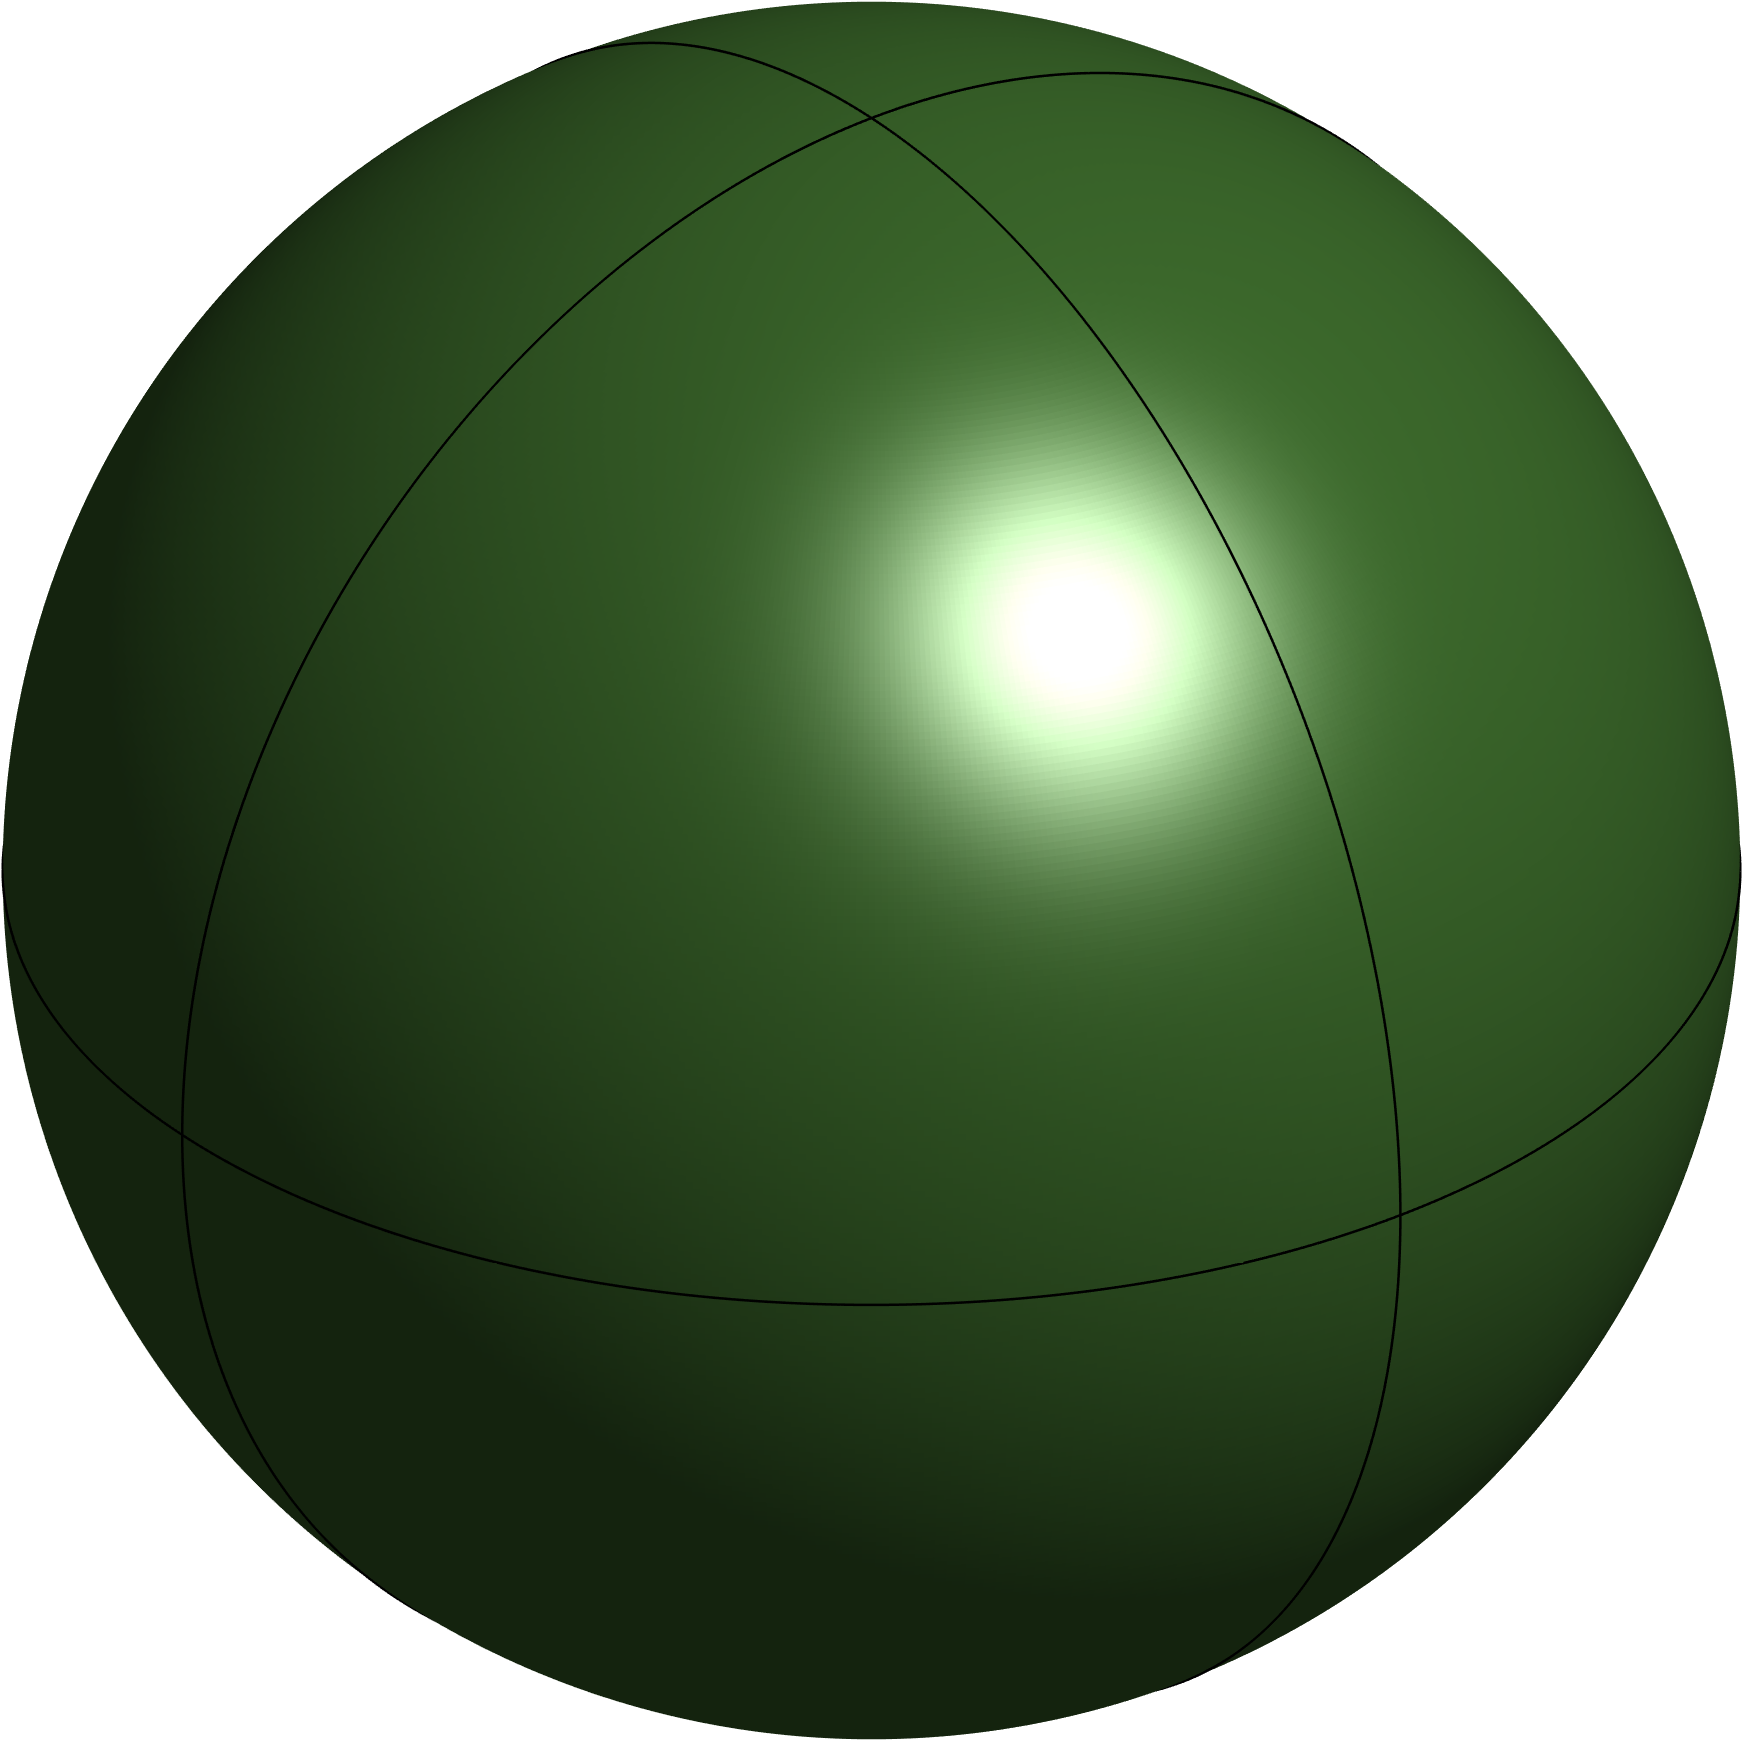
\includegraphics[width=\textwidth]{../../graphics/sphericalShell/sphericalShellMesh1_2_0}
		\caption{Exact geometry.}
	\end{subfigure}%
	\hspace*{0.11\textwidth}%   
	\begin{subfigure}[t]{0.26\textwidth}
		\centering
		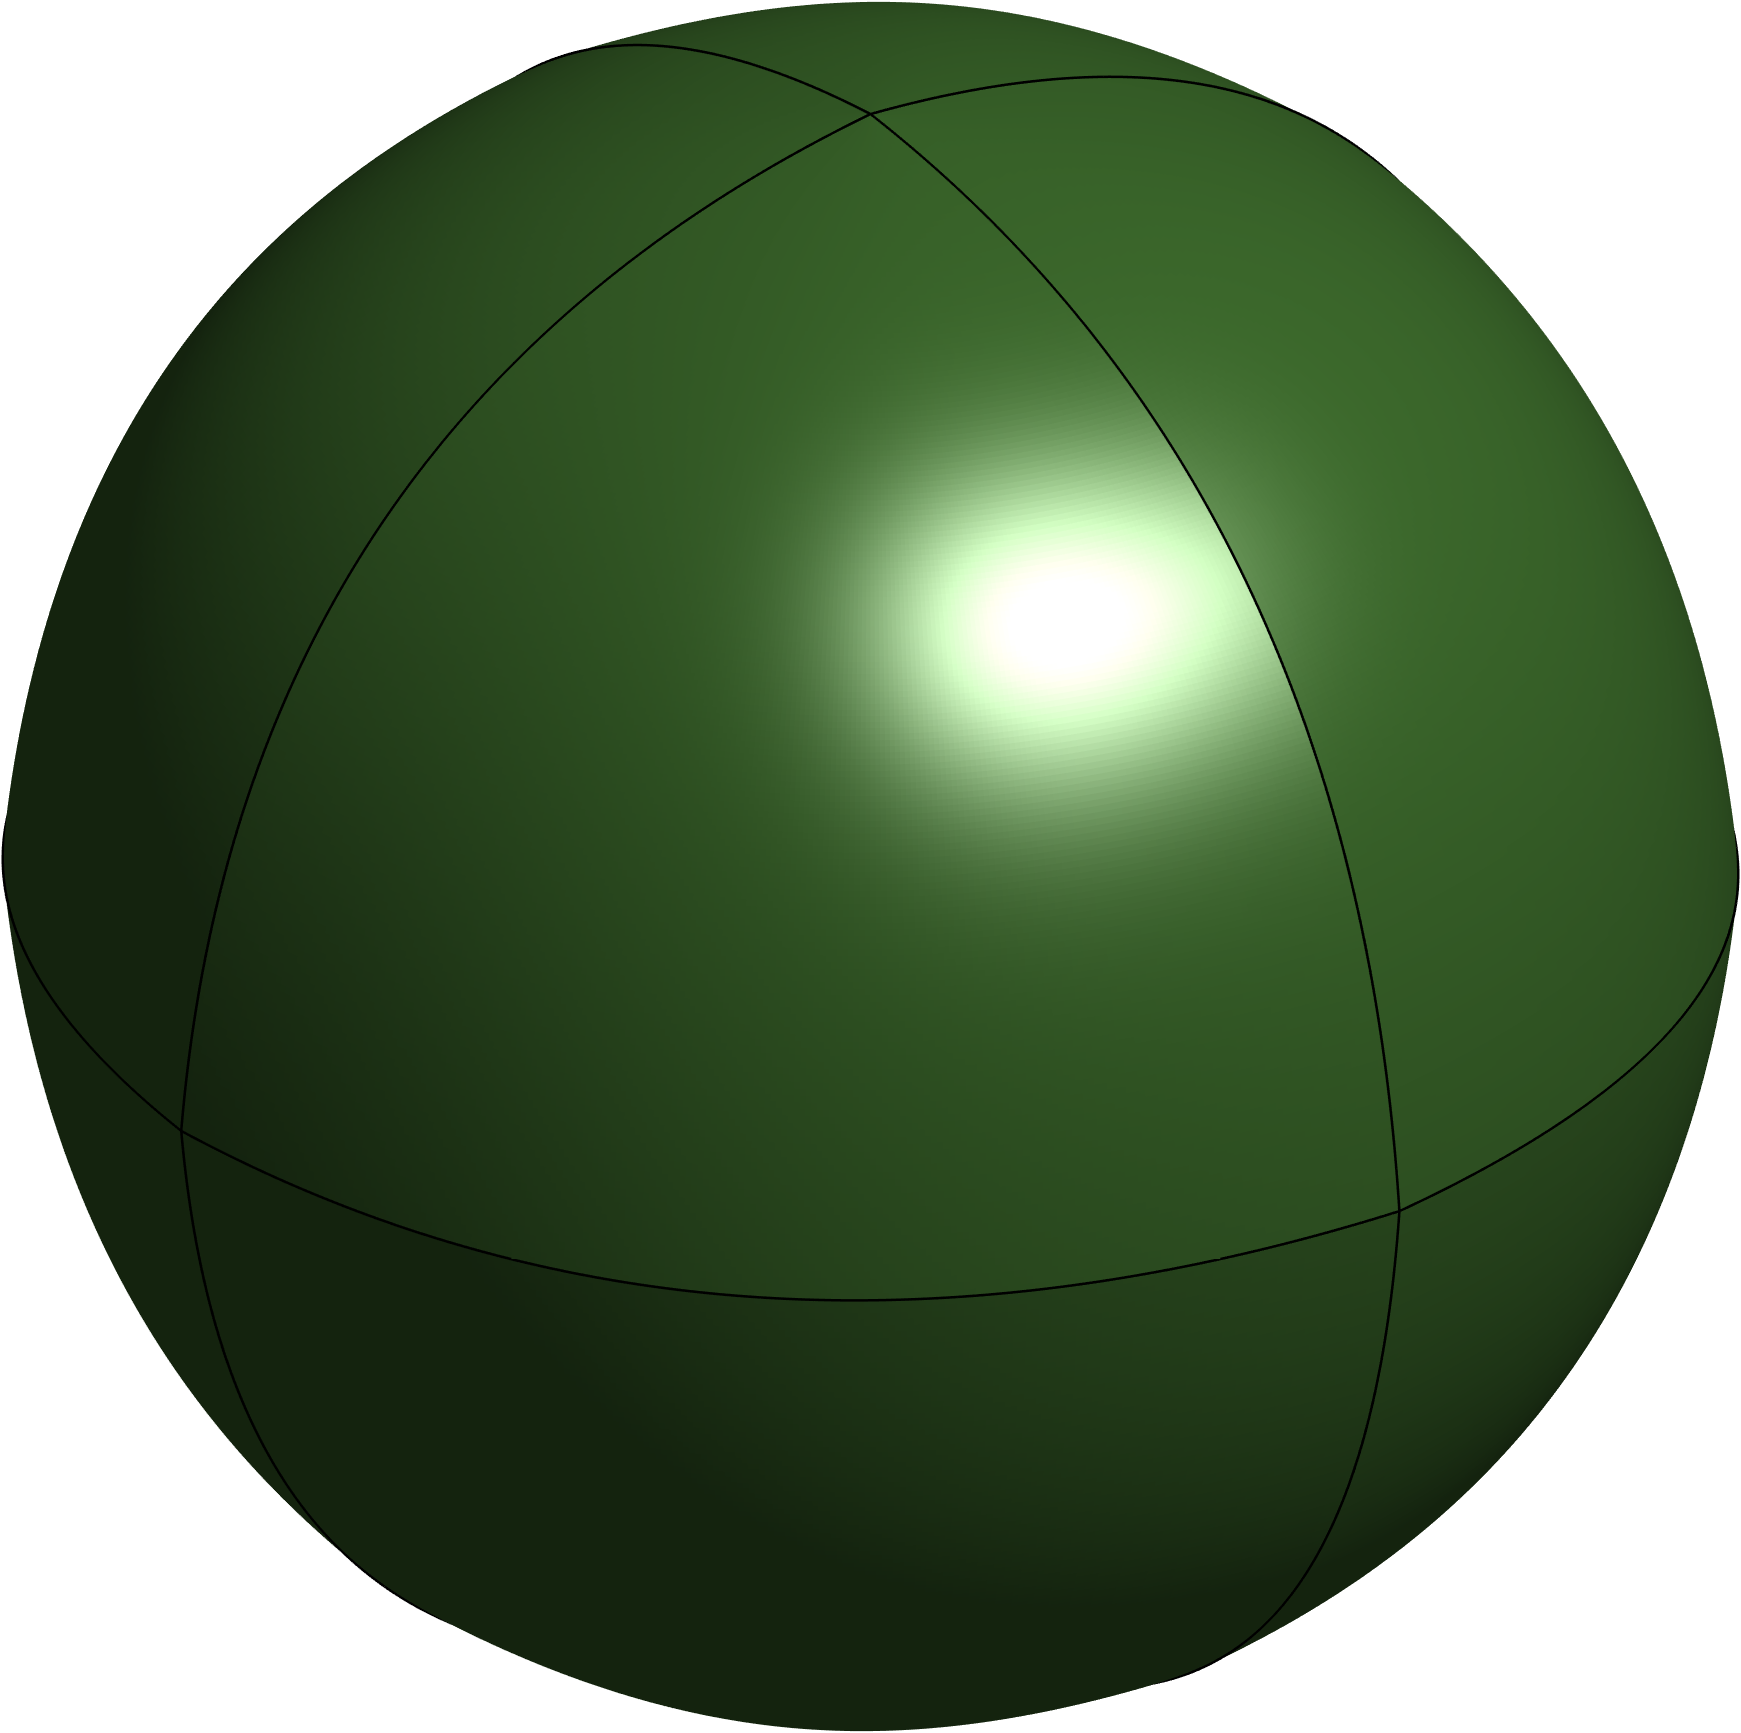
\includegraphics[width=\textwidth]{sphericalShellMesh1_2_FEM}
		\caption{Approximation using $\check{p}_\upxi=\check{p}_\upeta=2$.}
	\end{subfigure}%
	\hspace*{0.11\textwidth}%   
	\begin{subfigure}[t]{0.26\textwidth}
		\centering
		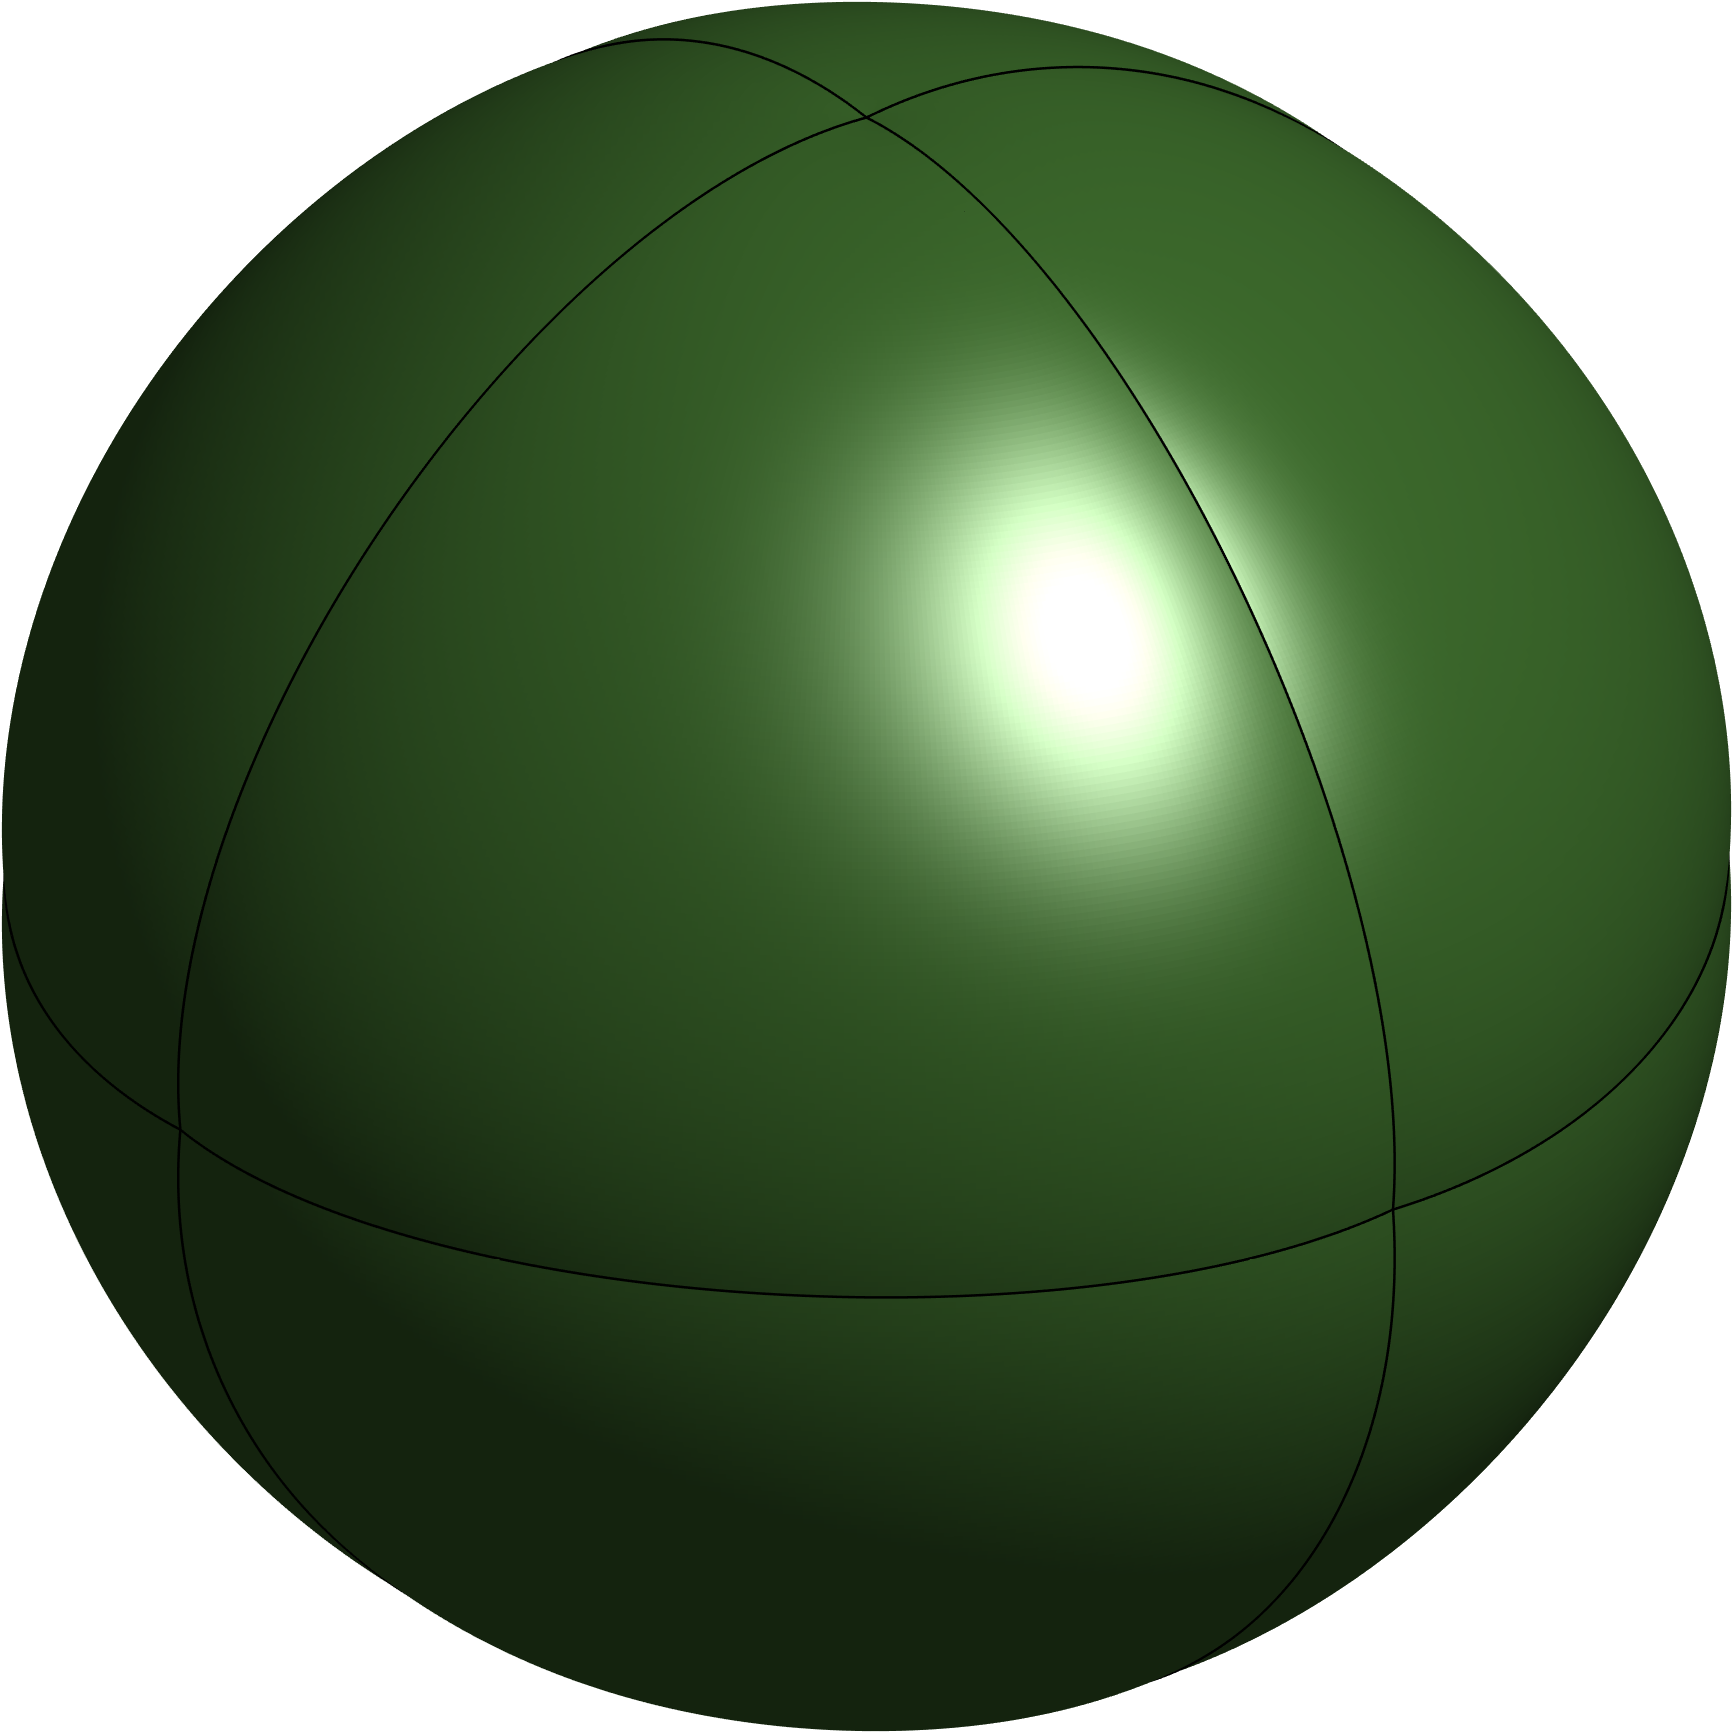
\includegraphics[width=\textwidth]{sphericalShellMesh1_3_FEM}
		\caption{Approximation using $\check{p}_\upxi=\check{p}_\upeta=3$.}
	\end{subfigure}
	\caption{Transformation of an exact NURBS parametrization of a spherical shell to a B-spline approximation of the same geometry.}
	\label{Fig2:NURBStoBsplineTransVis}
\end{figure}
